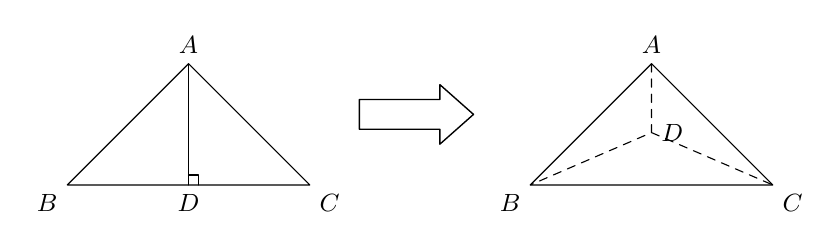
\begin{tikzpicture}[x=7mm,y=7mm,line cap=round,line join=round,every node/.style={font=\small}]
  % Folded isosceles right triangle: original shape at left, folded shape at right.
  \coordinate (A1) at (0,2.20);
  \coordinate (B1) at (-2.20,0);
  \coordinate (D1) at (0,0);
  \coordinate (C1) at (2.20,0);
  \draw (B1)--(A1)--(C1)--(B1);
  \draw (A1)--(D1);
  \draw (0.18,0)--(0.18,0.18)--(0,0.18);
  \node[above] at (A1) {$A$};
  \node[below left] at (B1) {$B$};
  \node[below] at (D1) {$D$};
  \node[below right] at (C1) {$C$};

  \draw[line width=.5pt] (3.10,1.01)--(4.56,1.01)--(4.56,.74)--(5.17,1.28)--(4.56,1.82)--(4.56,1.55)--(3.10,1.55)--cycle;

  \coordinate (B2) at (6.20,0);
  \coordinate (C2) at (10.60,0);
  \coordinate (A2) at (8.40,2.20);
  \coordinate (D2) at (8.40,.95);
  \draw (B2)--(A2)--(C2)--(B2);
  \draw[dash pattern=on 3pt off 2.5pt] (A2)--(D2)--(B2) (D2)--(C2);
  \node[above] at (A2) {$A$};
  \node[below left] at (B2) {$B$};
  \node[below right] at (C2) {$C$};
  \node[right] at (D2) {$D$};
\end{tikzpicture}
